%%%%%%%%%%%%%%%%%%%%%%%%%%%%%%%%%%%%%%%%%%%%%%%%%%%%%%%%%%%%%%%%%%%%%%%%%%%%%%%%%%%%%%%%%%%%%%%%%%%%
% Project Requirements Specification Report
% Authors: Michael Galliers and James Miller
% Course: CSC 440
%%%%%%%%%%%%%%%%%%%%%%%%%%%%%%%%%%%%%%%%%%%%%%%%%%%%%%%%%%%%%%%%%%%%%%%%%%%%%%%%%%%%%%%%%%%%%%%%%%%%

\documentclass[12pt]{article}
\usepackage[utf8]{inputenc}
\usepackage{graphicx}
\usepackage{float}
\usepackage{tocloft}
% Page margins
\usepackage[letterpaper, portrait, margin=1in]{geometry}

% Document configuration

% Section numbering
\renewcommand \thesection{\Roman{section}}
\renewcommand \thesubsection{\Alph{subsection}.}

% Environment config for requirements
%  - Configures formatting of the section heading and numbered, nested lists
\newenvironment{requirement}[1]
{
    % Format requirement sections (R1. ...)
    \renewcommand{\thesubsubsection}{R\arabic{subsubsection}.}
    % Format nested, numbered lists (1.1, 1.1.1, 1.1.1.1, ...)
    \renewcommand{\labelenumi}{
        \arabic{subsubsection}.\arabic{enumi}
    }
    \renewcommand{\labelenumii}{
        \arabic{subsubsection}.\arabic{enumi}.\arabic{enumii}
    }
    \renewcommand{\labelenumiii}{
        \arabic{subsubsection}.\arabic{enumi}.\arabic{enumii}.\arabic{enumiii}
    }
    \renewcommand{\labelenumiv}{
        \arabic{subsubsection}.\arabic{enumi}.\arabic{enumii}.\arabic{enumiii}.\arabic{enumiv}
    }
    % Create the subsubsection for the requirement
    \subsubsection{#1}
}
{}


% Set path to all graphics
\graphicspath{{figures/}{build/diagrams/}}

% Do paragraph indenting after section tags
\usepackage{indentfirst}

% Adjust space between numbers and headings in table of contents
\addtolength{\cftsecnumwidth}{12pt}
\addtolength{\cftsubsubsecnumwidth}{-10pt}


\author{Michael Galliers and James Miller}
\title{CSC 440 - Requirements Specification Report}


\begin{document}

\begin{titlepage}
\maketitle
\end{titlepage}

\newpage
    \tableofcontents
\newpage

\section{Introduction}
\subsection{Problem Statement}
As EKU college students, we the authors have firsthand experience with the difficulties of
grade/progress management. The tools already used by the college for grade management have their
flaws. Many professors either do not setup the grading categories and weights properly, or they
choose to not use BlackBoard for tracking grades at all. Also, BlackBoard does not have the ability
to give advanced insights for student grades other than simple weighted averages or totals.

Students can choose to manage their grades on their own, either using technology, such as
spreadsheets, or pen and paper. Students who do this are able to gain more insights into their
progress in courses, but it can be very time consuming to setup spreadsheets or do computations by
hand, especially when predicting grades needed on an assignment.

\subsection{Proposal}
As a solution to these problems, we propose a software system for grade and progress tracking. The
system shall have 2 main related components: one for grade tracking and one for major/concentration
progress tracking. The grade tracking system will allow students to easily enter and track their
grades across colleges, semesters, courses, and categories (homework, exams, etc.). Various views on
the user interface will display grades/scores using visual elements and animations, making it easy
for students to see how well they are doing.

The second component of the application is a progress tracker for majors and concentrations.
Information provided through the grade tracking feature, coupled with course requirements structures
will allow students to view their progress across multiple majors and concentrations.

\section{System Description}
The system shall have a user account management component to keep track of students, including the
ability to register, login, edit account, and logout. When a student logs into the system, the
student shall see a dashboard containing the most relevant information and navigation links. From
there, the student will also be able to access the system menu, allowing them to navigate to either
the grade tracking component or the progress tracking component.

\subsection{Grade Tracking Component}
\noindent
The grade tracking component shall have views for the following items:

\begin{enumerate}
    \item All semesters (root grade tracking view)
    \item Courses in a semester
    \item Details of a course (including categories and grade entries)
\end{enumerate}

The \textit{All Semesters} view shall allow the student to navigate to a particular semester,
add/remove a semester in which they are enrolled, and view statistics about his/her grades in that
semester.

The \textit{Courses} view shall display the courses that are in a particular semester. The student
shall be able to add/remove/edit courses, view statistics for grades in each course, and navigate
to any of the courses.

The \textit{Course Detail} view shall display all remaining details for a particular course. This
includes the statistics of a student's grades in the course, the grading categories of the course,
and the grade entries themselves. The student shall also have the ability to add/remove/edit
categories and grade entries.

\subsection{Progress Tracking Component}
\noindent
The progress tracking component shall allow students to track their progress across major
concentrations. This component shall have the following hierarchical views:

\begin{enumerate}
    \item Colleges (root progress tracking view)
    \item Majors
    \item Concentrations
    \item Concentration progress
\end{enumerate}

The \textit{Colleges} view shall display the colleges in which the student is enrolled and allow
him/her to navigate to the \textit{Majors} view for that college. The student shall also have the
ability to add/remove colleges which he/she is enrolled in.

The \textit{Majors} view shall display the majors of the college which was navigated from that the
student is enrolled in. The student shall be able to add/remove majors which he/she is enrolled in
and also navigate to the \textit{Concentrations} view for a particular major.

The \textit{Concentrations} view shall display \textbf{all} the concentrations of the major which
was navigated from, broken up into 2 sections: one for the concentration(s) the student in enrolled
in and one for all other concentrations. The student shall be able to add/remove concentrations
which they are enrolled in and navigate to the \textit{Concentration progress} view.

The \textit{Concentration progress} view shall display visuals for the student's progress in the
concentration, including overall progress and individual courses completed. This view shall be based
on courses the student has entered through the grade tracking component.

\section{System Requirements}
\subsection{Functional Requirements}
% \begin{requirement}{The system shall..1}


% \begin{enumerate}
%     \item Test item 1
%     \item Test item 2
%     \begin{enumerate}
%         \item Test item 1.1
%         \item Test item 1.2
%         \begin{enumerate}
%             \item Test item 1.1.1
%             \item Test item 1.1.2
%             \begin{enumerate}
%                 \item Test item 1.1.1.1
%                 \item Test item 1.1.1.2
%             \end{enumerate}
%         \end{enumerate}
%     \end{enumerate}
% \end{enumerate}


% \end{requirement}

% \begin{requirement}{The system shall..2}


% \begin{enumerate}
%     \item Test item 1
%     \item Test item 2
%     \begin{enumerate}
%         \item Test item 1.1
%         \item Test item 1.2
%         \begin{enumerate}
%             \item Test item 1.1.1
%             \item Test item 1.1.2
%             \begin{enumerate}
%                 \item Test item 1.1.1.1
%                 \item Test item 1.1.1.2
%             \end{enumerate}
%         \end{enumerate}
%     \end{enumerate}
% \end{enumerate}


% \end{requirement}

\subsection{Non-functional Requirements}

\subsection{Domain Requirements}

\begin{figure}[p!]
  \section{Use-case Diagram}
  \centering
  \includegraphics[width=0.8\linewidth]{use_case_diagram.pdf}
  \caption{Use-case Diagram}
\end{figure}

\section{Data Flow Diagrams}

\begin{figure}[p!]
  \subsection{Level 0 DFD}
  \centering
  \includegraphics[width=0.7\linewidth]{level_0_dfd.pdf}
  \caption{Level 0 DFD}
\end{figure}

\clearpage

% \section{Sequence Diagrams}

% \section{State Diagram}

% \section{Activity Diagrams}

\section{Database Design}

\begin{figure}[p!]
  \subsection{ER Schema}
  \centering
  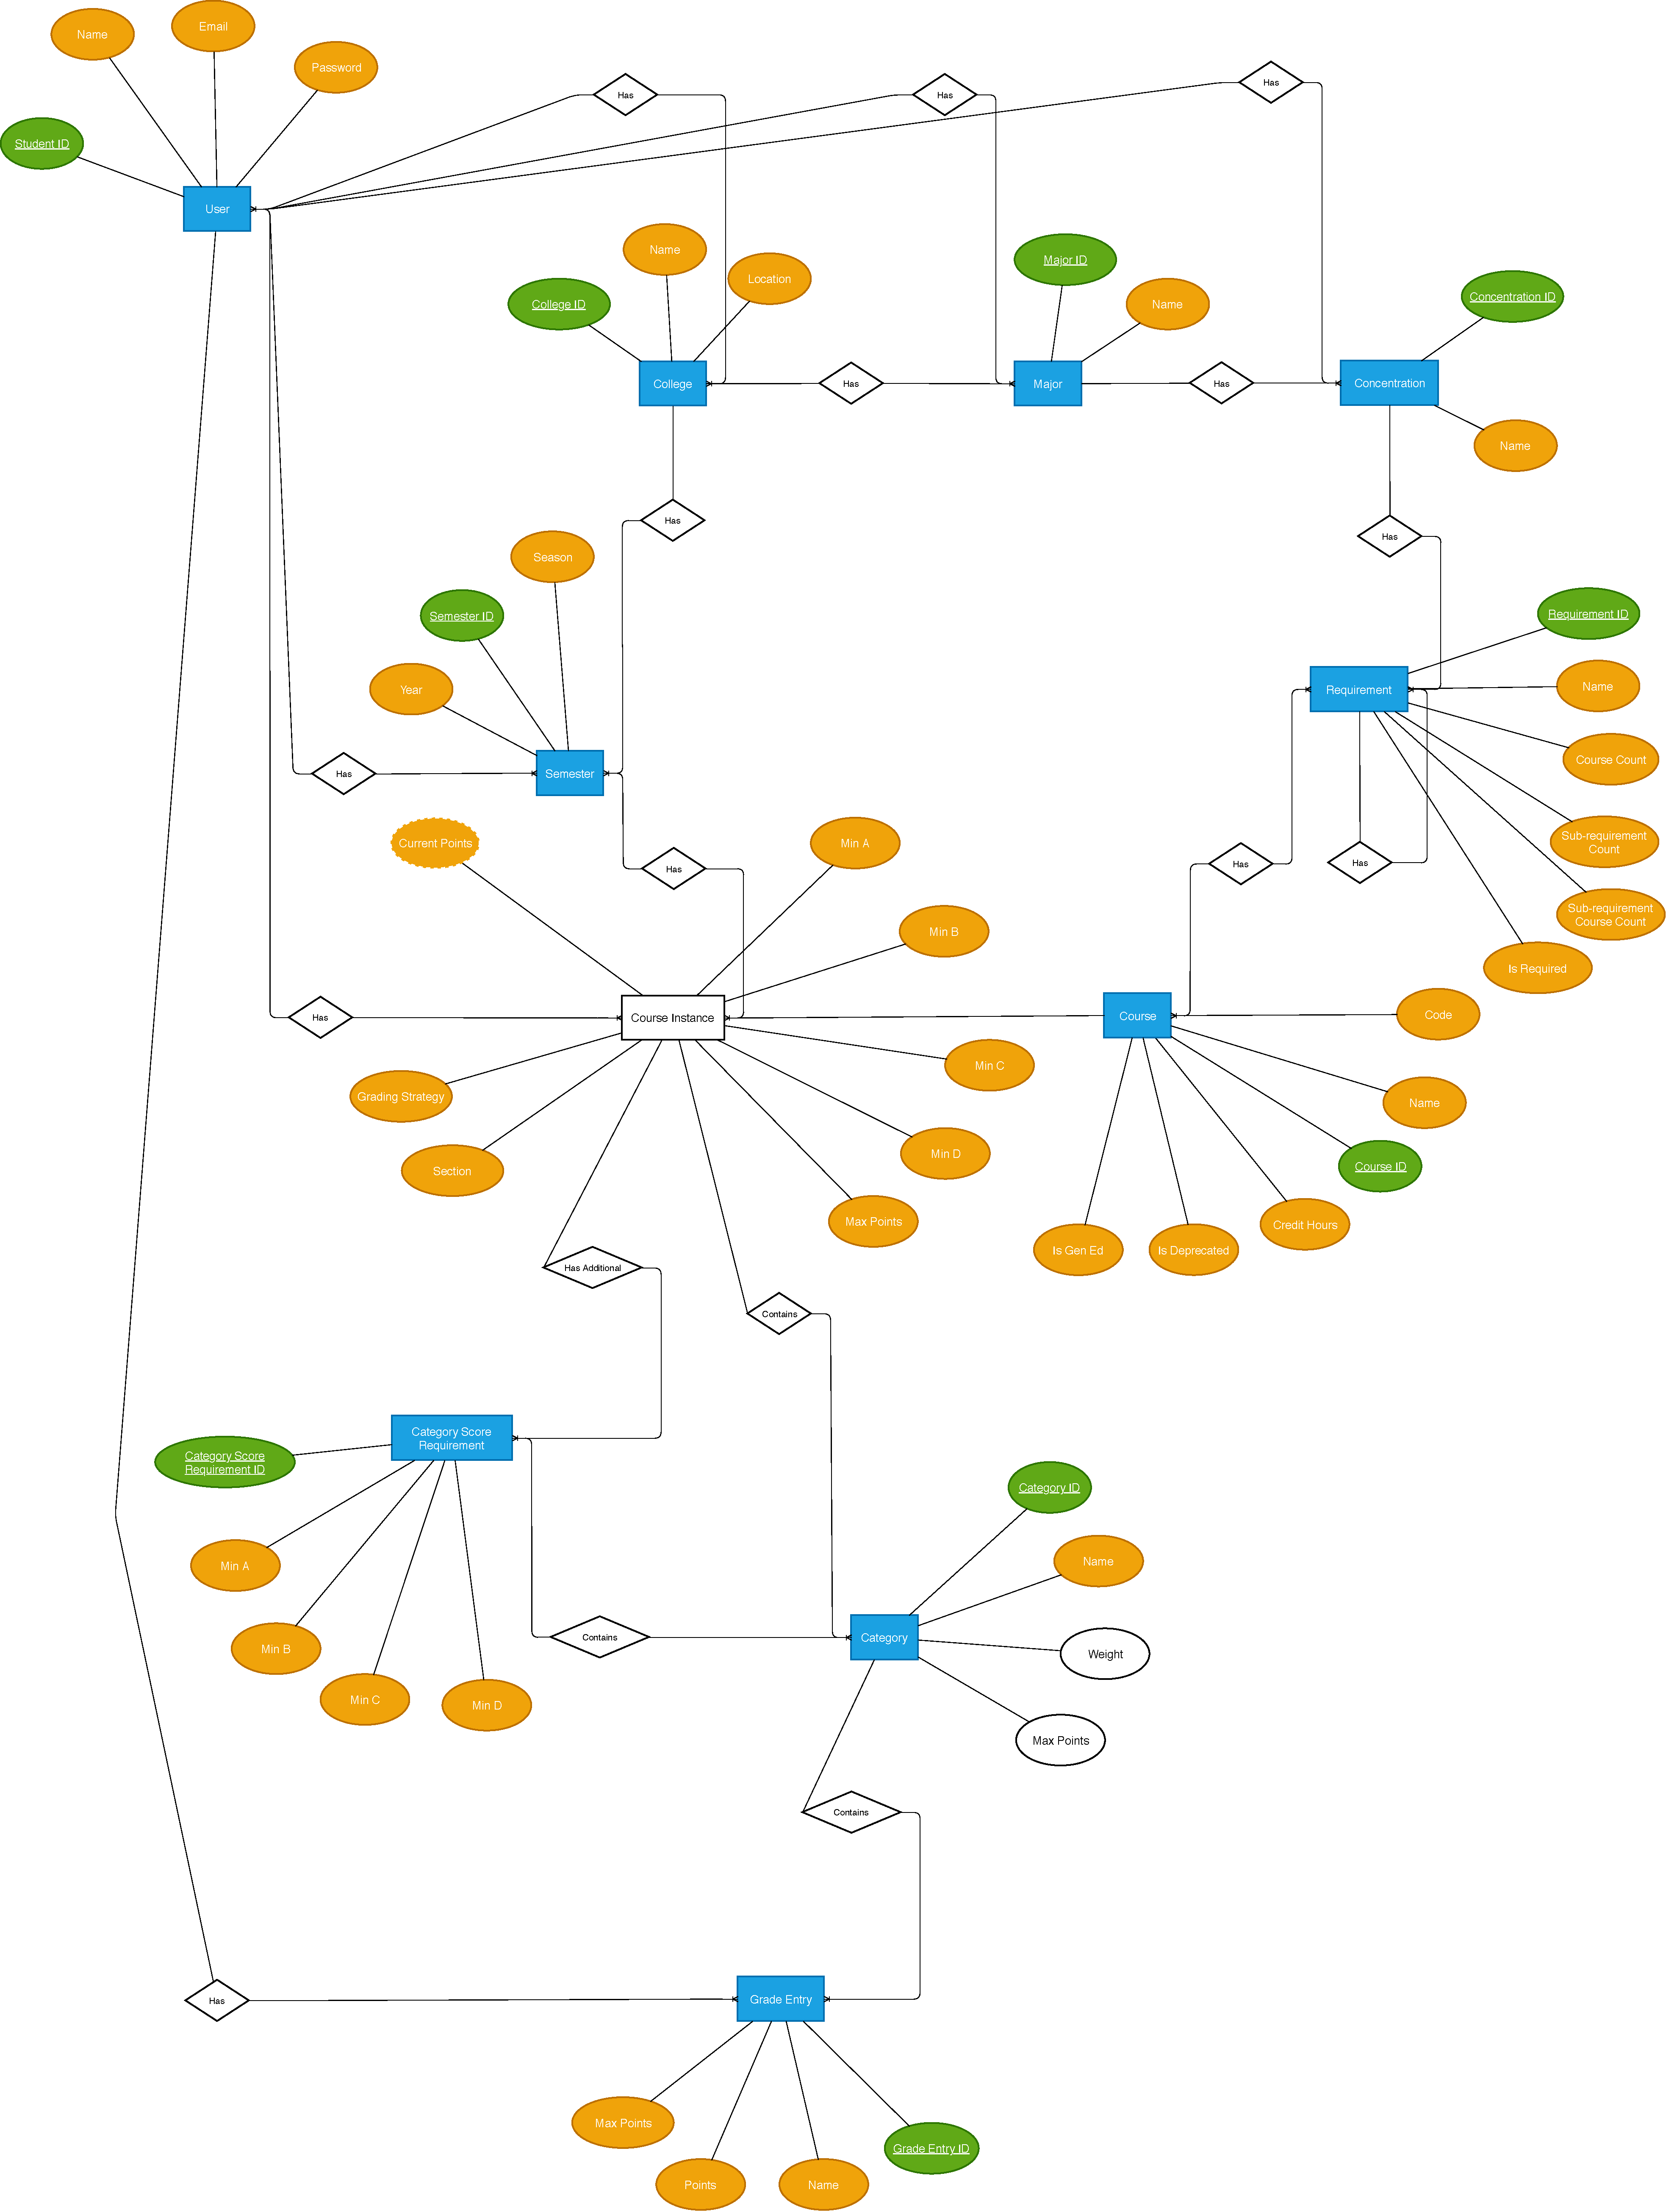
\includegraphics[width=\linewidth]{database_erd.pdf}
  \caption{Database ERD}
\end{figure}

\clearpage

\subsection{Table Schema}

\section{Conclusion}

\section{Dictionary}
\begin{itemize}
    \item \textbf{Semester}: A single semester of education consisting of courses. Each semester can
    be associated with a different educational institution; consistency is not required.
    \item \textbf{Course}: Any educational course/class occurring within a particular semester.
    \item \textbf{Section}: An equally weighted or logically grouped collection of material within a
    particular course (e.g. Homework, Tests, etc.).
    \item \textbf{Grade Entry}: A graded piece of material associated with a particular section 
    (e.g. Homework 2, Exam 1, etc.).
    \item \textbf{studentName} (string): Name of a student
    \item \textbf{studentEmail} (string): Email of a student
    \item \textbf{studentUsername} (string): Username of a student
    \item \textbf{studentPassword} (string): Password of a student
    \item \textbf{student} (Student): Student object, composed of studentName, studentEmail,
          studentUsername, studentPassword
    \item \textbf{semester} (Semester): Semester object
    \item \textbf{course} (Course): Course object
    \item \textbf{category} (Category): Category object
    \item \textbf{gradeEntry} (GradeEntry): GradeEntry object
    \item \textbf{gradeEntry} (GradeEntry): GradeEntry object
\end{itemize}

\end{document}
